\cleardoublepage
\clearpage{}

%[Lo que va en el índice]{Lo que va en el documento}
\chapter[Implementación y experimentación]{Implementación y experimentación}

\section{KnowSeq}
Tras realizar las ejecuciones de \textit{KnowSeq} en los tres sistemas de archivos se obtuvieron los resultados que aparecen en el anexo \ref{resultados_knowseq}. Se han seguido las pautas especificadas en la metodología. \\

En primer lugar se creó la partición /dev/sda1 en el disco destinado a las pruebas. Acto seguido se creó y se montó el sistema de archivos. Tras esto el siguiente paso conseistía en  copiar los archivos necesarios para la ejecución de \textit{KnowSeq} en el disco y tras ello lanzar el script que automatiza la ejecución de la prueba y la recogida de datos a través de \textit{iowatcher}. Estos pasos se repitieron para cada uno de los tres sistemas de archivos.\\

La salida de \textit{iowatcher} consiste en una gráfica de la productividad en MB/s a través del tiempo y un archivo de texto con los ítems medidos, cuyo formato es poco amigable. La salida de \textit{iowatcher} para los tres sistemas es la que se muestran a continuación.\\ 

\begin{figure}[H]
    \centering
    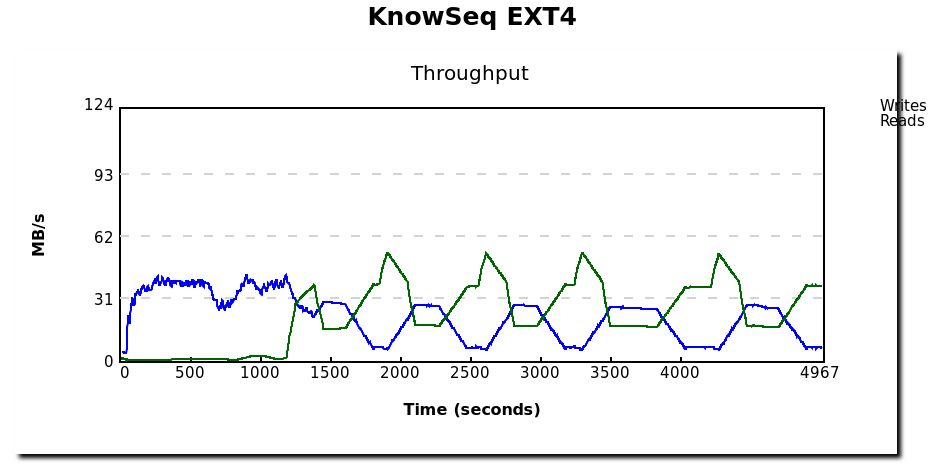
\includegraphics[scale=0.35]{doc/assets/images/Capitulo4/Knowseq/knowseq_ext4.png}
    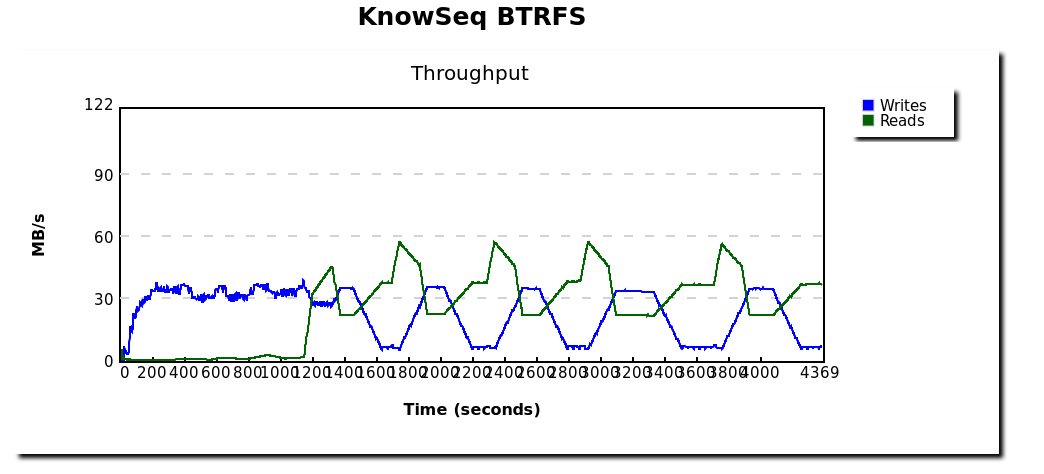
\includegraphics[scale=0.35]{doc/assets/images/Capitulo4/Knowseq/knowseq_btrfs.png}
    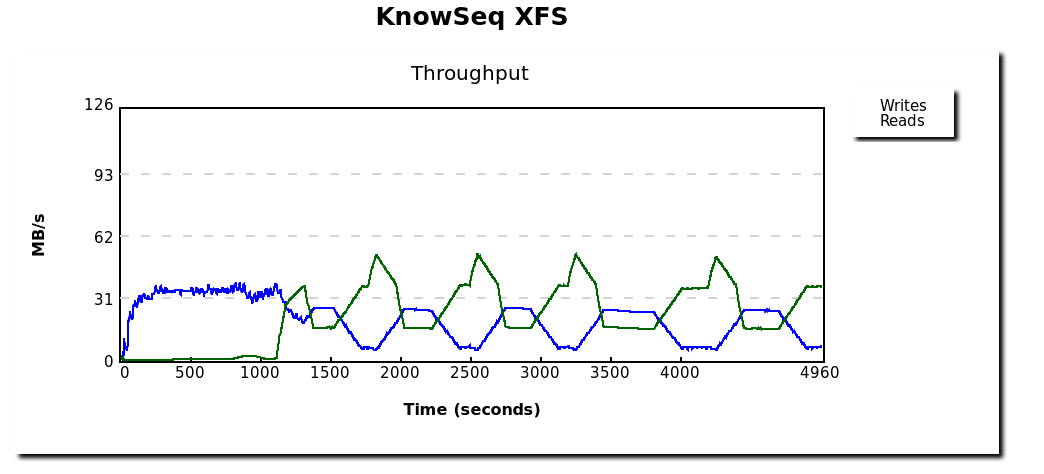
\includegraphics[scale=0.35]{doc/assets/images/Capitulo4/Knowseq/knowseq_xfs.png}
    \caption{Gráfica del rendimiento en \textit{KnowSeq} para cada sistema de archivos}
    \label{fig:my_label}
\end{figure}

Como se observa en las imágenes el patrón de velocidad de lecturas/escrituras es similar, esta situación puede ayudar a determinar que las pruebas han sido ejecutadas de forma correcta y que el programa en todos los casos realizó las mismas operaciones.

El siguiente paso consiste en transformar el archivo de texto que proporciona \textit{iowatcher} como salida ya que dicho documento no se encuentra en formato legible por el ser humano, para ello se utiliza \textit{blkparse}. La salida de \textit{blkparse}, entre otros muchos datos, nos proporciona la productividad en KiB/s. Con el fin de trabajar con unas unidades más usuales se decide transformar a MB/s y anotarlo en una hoja de cálculo y tras ello se calcula la media y desviación. Tal y como se puede ver en la tabla.

\begin{table}[H]\centering 
\caption{Productividad de la prueba KnowSeq para EXT4, BTRFS y XFS} 
\scriptsize
\begin{tabular}{lrrrrrrr}\toprule
\textbf{Nº Ejecución} &\multicolumn{2}{c}{\textbf{EXT4}} &\multicolumn{2}{c}{\textbf{BTRFS}} &\multicolumn{2}{c}{\textbf{XFS}} \\\cmidrule{1-7}
&\textbf{Lectura} &\textbf{Escritura} &\textbf{Lectura} &\textbf{Escritura} &\textbf{Lectura} &\textbf{Escritura} \\\midrule
\textbf{1} &24.682 &21.703 &28.041 &24.574 &24.567 &21.533 \\
\textbf{2} &24.108 &21.143 &28.045 &24.568 &24.352 &21.402 \\
\textbf{3} &23.955 &20.977 &27.676 &24.258 &24.543 &21.570 \\
\textbf{4} &24.464 &21.498 &28.280 &24.795 &24.496 &21.529 \\
\textbf{} & & & & & & \\
\textbf{Promedio} &24.303 &21.330 &28.010 &24.549 &24.489 &21.508 \\
\textbf{Desviación} &0.331 &0.330 &0.250 &0.221 &0.096 &0.073 \\
\bottomrule
\end{tabular}
\end{table}
A partir de los datos de la tabla anterior podemos generar una gráfica con la media de la productividad.

\begin{figure}[H] 
    \centering
    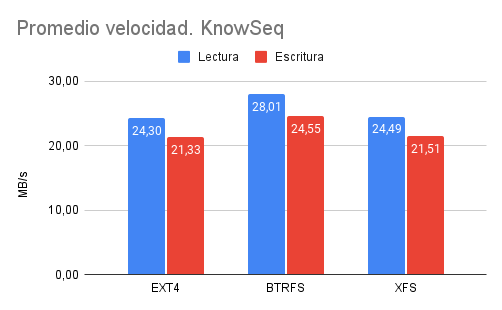
\includegraphics[scale=0.6]{doc/assets/images/Capitulo4/Knowseq/promknow.png}
    \caption{Productividad en MB/s de las pruebas usando KnowSeq y tres sistemas de archivos.}
    \label{aa}
\end{figure}

Se podría pensar que viendo la imagen \ref{aa} es suficiente para afirmar que BTRFS es mejor para el trabajo que realiza \textit{KnowSeq}. Pero surgen varias cuestiones ¿Es realmente mas productivo, o simplemente es casualidad o error en las mediciones?  ¿El utilizar un sistema de archivos u otro tiene que ver con la mejora de productividad?\\

Se decide por tanto realizar dos tests Anova del cual se habló en la sección \ref{anova_section}. Si tanto para lectura como para escritura se llega a la conclusión de que el factor sistema de archivos importa y es determinante.\\

Partimos de la hipótesis de que el rendimiento en lectura es igual para los tres sistemas de archivos y que el sistema de archivos no influye. Definimos la prueba al 95\% de confianza, es decir, $\alpha = 0.05$.\\

Generamos un csv con los datos en MB/s para cada sistema de archivos en lecturas y ejecutamos el script \ref{Anova.py} para el cálculo del \textit{p-value}. Obtenemos que el p-valor es $6.8424*10^{-9}$.\\

Para confirmar dicho resultado se repite el test con los mismos datos en la hoja de cálculo, cuyo resultado se refleja en la siguiente tabla. Se observa que obtenemos el mismo el p-valor. 

\begin{table}[!htp]\centering
\scriptsize
\begin{tabular}{lrrrrrrr}\toprule
Source of Variation &SS &df &MS &F &P-value &F crit \\\midrule
Between Groups &34.908 &2.0 &17.4541 &289.0014 &0.000000006842 &4.2565 \\
Within Groups &0.544 &9.0 &0.0604 & & & \\
& & & & & & \\
Total &35.452 &11.0 & & & & \\
\bottomrule
\end{tabular}
\caption{Resultado test Anova para las lecturas de \textit{KnowSeq}}\label{tab: }
\end{table}

Procedemos de la misma manera para realizar el test Anova para escritura con el objetivo de obtener un p-valor. Partimos de la hipótesis de que el rendimiento en escritura es igual en los tres sistemas de archivos. Ejecutamos el test Anova, y el resultado obtenido es el que se muestra en la siguiente tabla.

\begin{table}[!htp]\centering
\scriptsize
\begin{tabular}{lrrrrrrr}\toprule
Source of Variation &SS &df &MS &F &P-value &F crit \\\midrule
Between Groups &26.1819 &2 &13.0909 &240.5899 &0.00000001539899 &4.2565 \\
Within Groups &0.4897 &9 &0.0544 & & & \\
& & & & & & \\
Total &26.6716 &11 & & & & \\
\bottomrule
\end{tabular}
\caption{Resultado test Anova para las escrituras de \textit{KnowSeq}}\label{tab: }
\end{table}

Para finalizar se discutirán los resultados de los tests. Como en ambos test el \textit{p-value} es menor que $\alpha$ se rechazan ambas hipótesis nulas que se definieron al principio.\\

Se llega a la conclusión de que el rendimiento tanto en lectura como en escritura no es equivalente entre sistemas de ficheros. Es decir, existen diferencias significativas entre los sistemas de archivos para la ejecución de \textit{KnowSeq}. Por tanto se puede afirmar que BTRFS para la prueba KnowSeq es más productivo.

\section{Iozone}
Siguiendo las consideraciones que se detallaron en la sección \ref{metodologia_iozone} se ejecutaron los test. Desafortunadamente, debido al tiempo que tomaría y a la gran cantidad de datos que ello generaría se decidió repetir la prueba sólo cuatro veces, puesto que la desviación entre pruebas no es excesivamente alta. Es decir, se ha tenido que prescindir de la fórmula \ref{eqn:n-ejecuciones} para calcular el número de ejecuciones.\\

La salida de \textit{iozone} se presenta en formato tabla. La productividad depende del tamaño de archivo y del \textit{record length}. Con esta situación cabe preguntarse si las variaciones de dichos tamaños afectan realmente al rendimiento o no. Por ello se realiza un test Anova para comprobarlo.

\subsection{Test Anova para tamaño de archivo}
Para la realización de este test se realizaron 4 mediciones para tres configuraciones distintas de \textit{record size}. Por lo tanto se necesitan tres test, uno para cada tamaño de \textit{record size}.  Los resultados de dichas mediciones se pueden consultar en el Anexo \ref{tab:tabla_salida_anova_archivo}. Tras generar las tablas, se procede a ejecutar los test Anova. Antes se necesita especificar cual es la hipótesis nula, en este caso, la hipótesis es que el rendimiento es  igual para cualquier tamaño de archivo. La salida obtenida es la siguiente. 

\begin{table}[H]\centering
\scriptsize
\begin{tabular}{lrrrrrrr}\toprule
Source of Variation &SS &df &MS &F &P-value &F crit \\\midrule
Between Groups &16353394702915.422 &13 &1257953438685.8018 &89.29416792 &0 &1.9612184003 \\
Within Groups &591685276360.5 &42 &14087744675.25 & & & \\
& & & & & & \\
Total &16945079979275.922 &55 & & & & \\
\bottomrule
\end{tabular}
\caption{Resultado test Anova para comprobar si el tamaño de archivo es un factor que afecta a la productividad con un tamaño de \textit{record size de 64KB}}\label{tab: }
\end{table}

\begin{table}[H]\centering
\scriptsize
\begin{tabular}{lrrrrrrr}\toprule
Source of Variation &SS &df &MS &F &P-value &F crit \\\midrule
Between Groups &13060330768231.422 &13 &1004640828325.494 &61.457186809122 &0 &1.96121840 \\
Within Groups &686574133644 &42 &16347003182 & & & \\
& & & & & & \\
Total &13746904901875.422 &55 & & & & \\
\bottomrule
\end{tabular}
\caption{Resultado test Anova para comprobar si el tamaño de archivo es un factor que afecta a la productividad con un tamaño de \textit{record size de 1024KB}}\label{tab: }
\end{table}

\begin{table}[H]\centering
\scriptsize
\begin{tabular}{lrrrrrrr}\toprule
Source of Variation &SS &df &MS &F &P-value &F crit \\\midrule
Between Groups &12138841872010.5 &9 &1348760208001.1667 &173.4900496764 &0 &2.21069698 \\
Within Groups &233228397337.5 &30 &7774279911.25 & & & \\
& & & & & & \\
Total &12372070269348 &39 & & & & \\
\bottomrule
\end{tabular}
\caption{Resultado test Anova para comprobar si el tamaño de archivo es un factor que afecta a la productividad con un tamaño de \textit{record size de 16384KB}}\label{tab: }
\end{table}

Como para los tres tamaños de \textit{record size} $p-value < 0.05$ se rechaza la hipótesis planteada. El tamaño de archivo \textbf{si} es un factor que influye en la productividad.

\subsection{Test Anova para \textit{record size}}
De igual manera se procede en este caso. Fijamos tres tamaños de archivos, en este caso 512MB, 2GB y 8GB. Los tamaños de record size van a ser los que varíen. Igual que en el test anterior se ha repetido la prueba 4 veces para cada tamaño de archivo. La hipótesis nula es que el \textit{record size} no es un factor que influya en el rendimiento. Los resultados para los tres test son los siguientes:

\begin{table}[H]\centering
\scriptsize
\begin{tabular}{lrrrrrrr}\toprule
Source of Variation &SS &df &MS &F &P-value &F crit \\\midrule
Between Groups &7157416779626.656 &11 &650674252693.3324 &188.781965827 &0 &2.066608478 \\
Within Groups &124081095322 &36 &3446697092.2777777 & & & \\
& & & & & & \\
Total &7281497874948.656 &47 & & & & \\
\bottomrule
\end{tabular}
\caption{Resultado test Anova para comprobar si el tamaño de \textit{record size} es un factor que afecta a la productividad con un tamaño de archivo de 512MB}\label{tab: }
\end{table}

\begin{table}[H]\centering

\scriptsize
\begin{tabular}{lrrrrrrr}\toprule
Source of Variation &SS &df &MS &F &P-value &F crit \\\midrule
Between Groups &653116815773.2305 &11 &59374255979.38459 &5.2127172 &0.00007428 &2.0666084 \\
Within Groups &410049713763.25 &36 &11390269826.756945 & & & \\
& & & & & & \\
Total &1063166529536.4805 &47 & & & & \\
\bottomrule
\end{tabular}
\caption{Resultado test Anova para comprobar si el tamaño de \textit{record size} es un factor que afecta a la productividad con un tamaño de archivo de 2GB}\label{tab: }
\end{table}

\begin{table}[!htp]\centering

\scriptsize
\begin{tabular}{lrrrrrrr}\toprule
Source of Variation &SS &df &MS &F &P-value &F crit \\\midrule
Between Groups &541800093953.917 &11 &49254553995.81064 &27.175544410 &3.619327e-14 &2.06660847825 \\
Within Groups &65248515984 &36 &1812458777.33333 & & & \\
& & & & & & \\
Total &607048609937.917 &47 & & & & \\
\bottomrule
\end{tabular}
\caption{Resultado test Anova para comprobar si el tamaño de \textit{record size} es un factor que afecta a la productividad con un tamaño de archivo de 8GB}\label{tab: }
\end{table}


Los p-valores en los tres casos son menores que el grado de significatividad $\alpha = 0,05$ por lo que en los tres casos rechazamos la hipótesis nula. El tamaño de \textit{record size} afecta a la productividad.

\subsection{Test Anova para Sistema de Archivos}
Para la realización de los test siguientes se han seguido las siguientes pautas.
\begin{itemize}
    \item Cuatro repeticiones por tamaño de \textit{record length}.
    \item Se realiza la prueba para seis operaciones (read/re-read, write/re-write, random-read/random-write).
    \item Tamaños de archivo de 200MB, 400MB, 800MB, 1.6GB, 3.2GB y 6GB.
    \item Tamaños de \textit{record length} de 4KB, 256KB, 1024KB y 16384KB.
    \item En las operaciones \textit{random read / random write} para tamaños de \textit{record size} de 4KB el tamaño de archivo máximo es 3.2GB y no 6GB, debido posiblemente, a un bug de \textit{iozone} que imposibilita acabar el test.
\end{itemize}

El objetivo consiste en analizar para cada una de las operaciones si el sistema de archivos afecta al rendimiento para ello se han fijado tamaño de archivo y \textit{record length} concretos. En resumen se han ejecutado pruebas para todas las combinaciones de operaciones, tamaño de archivos y tamaño de \textit{record length} anteriormente citadas. Se realizarán tests Anova utilizando dichas salidas. Los resultados de ejecutar iozone para cada test se encuentran en el anexo \ref{tablas_anova_sa}.\\



Para cada uno de los tests que se van a realizar a continuación la hipótesis nula es que el factor Sistema de Archivos \textbf{no} influye en el rendimiento. Para cada una de las operaciones hay seis test Anova, uno por cada tamaño de archivo. Los resultados de los tests se encuentran en el anexo \ref{tablas_anova_sa_por_operacion}
\subsubsection{Test Anova para factor Sistema de Archivos: \textit{record length} 4KB}

\subsubsection{Read}
\begin{table}[!htp]\centering
\scriptsize
\begin{tabular}{lrrrrrrr}\toprule
&200MB &400MB &800MB &1.6GB &3.2GB &6GB \\\midrule
p-value &0.000650 &0.0009706 &0.0005921 &0.0040223 &0.0098294 &0.0020086 \\
\bottomrule
\end{tabular}
\caption{P-valores para la operación \textit{read}.}\label{tab: }
\end{table}

Cómo los p-valores para todos los tamaños son menores que $\alpha$ = 0,05 podemos rechazar la hipótesis nula. El sistema de archivos influye en el rendimiento si realizamos operaciones de lectura. 

\subsubsection{Re-read}
\begin{table}[!htp]\centering
\scriptsize
\begin{tabular}{lrrrrrrr}\toprule
&200MB &400MB &800MB &1.6GB &3.2GB &6GB \\\midrule
p-value &0.000000848 &0.0000644 &0.0000029 &0.0000003 &0.0000013 &0.0005714 \\
\bottomrule
\end{tabular}
\caption{P-valores para la operación \textit{Re-read}.}\label{tab: }
\end{table}

Cómo los p-valores para todos los tamaños son menores que $\alpha$ = 0,05 podemos rechazar la hipótesis nula. El sistema de archivos influye en el rendimiento si realizamos operaciones de re-lectura. 


\subsubsection{Write}
\begin{table}[!htp]\centering
\scriptsize
\begin{tabular}{lrrrrrrr}\toprule
&200MB &400MB &800MB &1.6GB &3.2GB &6GB \\\midrule
p-value &0.0000860421 &0.0000156881 &0.0000020634 &0.02406280890 &0.000000042 &0.000003243 \\
\bottomrule
\end{tabular}
\caption{P-valores para la operación \textit{Write}.}\label{tab: }
\end{table}

Cómo los p-valores para todos los tamaños son menores que $\alpha$ = 0,05 podemos rechazar la hipótesis nula. El sistema de archivos influye en el rendimiento si realizamos operaciones de escritura. 

\subsubsection{Re-Write}
\begin{table}[!htp]\centering
\scriptsize
\begin{tabular}{lrrrrrrr}\toprule
&200MB &400MB &800MB &1.6GB &3.2GB &6GB \\\midrule
p-value &0.0000026 &0.0000024 &0.0000004 &0.0037634 &0.0000044 &0.0003532 \\
\bottomrule
\end{tabular}
\caption{P-valores para la operación \textit{Re-Write}.}\label{tab: }
\end{table}

Cómo los p-valores para todos los tamaños son menores que $\alpha$ = 0,05 podemos rechazar la hipótesis nula. El sistema de archivos influye en el rendimiento si realizamos operaciones de re-escritura. 

\subsubsection{Random-Read}
\begin{table}[!htp]\centering
\scriptsize
\begin{tabular}{lrrrrrrr}\toprule
&200MB &400MB &800MB &1.6GB &3.2GB \\\midrule
p-value &0.347155429 &0.241347798 &0.381537303 &0.264937379 &0.403343572 \\
\bottomrule
\end{tabular}
\caption{P-valores para la operación \textit{Random-Read}.}\label{tab: }
\end{table}

Cómo los p-valores para todos los tamaños son mayores que $\alpha$ = 0,05 podemos confirmar la hipótesis nula. El rendimiento del sistema de archivos es equivalente si realizamos operaciones de lectura aleatoria. 

\subsubsection{Random-Write}
\begin{table}[!htp]\centering
\scriptsize
\begin{tabular}{lrrrrrrr}\toprule
&200MB &400MB &800MB &1.6GB &3.2GB \\\midrule
p-value &0.04763 &0.04296 &0.03591 &0 &0.04148 \\
\bottomrule
\end{tabular}
\caption{P-valores para la operación \textit{Random-Write}.}\label{tab: }
\end{table}

Cómo los p-valores para todos los tamaños son menores que $\alpha$ = 0,05 podemos rechazar la hipótesis nula. El sistema de archivos influye en el rendimiento si realizamos operaciones de escritura aleatoria. 














\subsubsection{Test Anova para factor Sistema de Archivos: \textit{record length} 256KB}

\subsubsection{Read}
\begin{table}[!htp]\centering
\scriptsize
\begin{tabular}{lrrrrrrr}\toprule
&200MB &400MB &800MB &1.6GB &3.2GB &6GB \\\midrule
p-value &0.00008661 &0.00012866 &0.00027670 &0.01556616 &0.04768246 &0.04429488 \\ \\
\bottomrule
\end{tabular}
\caption{P-valores para la operación \textit{read}.}\label{tab: }
\end{table}

Cómo los p-valores para todos los tamaños son menores que $\alpha$ = 0,05 podemos rechazar la hipótesis nula. El sistema de archivos influye en el rendimiento si realizamos operaciones de lectura. 

\subsubsection{Re-read}
\begin{table}[!htp]\centering
\scriptsize
\begin{tabular}{lrrrrrrr}\toprule
&200MB &400MB &800MB &1.6GB &3.2GB &6GB \\\midrule
p-value &0.00001505 &0.00000678 &0.00000128 &0.00000720 &0.00000078 &0.00137099 \\
\bottomrule
\end{tabular}
\caption{P-valores para la operación \textit{Re-read}.}\label{tab: }
\end{table}

Cómo los p-valores para todos los tamaños son menores que $\alpha$ = 0,05 podemos rechazar la hipótesis nula. El sistema de archivos influye en el rendimiento si realizamos operaciones de re-lectura. 


\subsubsection{Write}
\begin{table}[!htp]\centering
\scriptsize
\begin{tabular}{lrrrrrrr}\toprule
&200MB &400MB &800MB &1.6GB &3.2GB &6GB \\\midrule
p-value &8.518119543055036e-11 &0.0000000049 &7.12607750585903e-12 &0.0000004213 &0.0000015795 &0.0000000003 \\
\bottomrule
\end{tabular}
\caption{P-valores para la operación \textit{Write}.}\label{tab: }
\end{table}

Cómo los p-valores para todos los tamaños son menores que $\alpha$ = 0,05 podemos rechazar la hipótesis nula. El sistema de archivos influye en el rendimiento si realizamos operaciones de escritura. 
 \newpage
\subsubsection{Re-Write}
\begin{table}[!htp]\centering
\scriptsize
\begin{tabular}{lrrrrrrr}\toprule
&200MB &400MB &800MB &1.6GB &3.2GB &6GB \\\midrule
p-value &0.0000084376 &3.3896164941e-7 &2.1347738021e-7 &5.5088662809e-7 &0.0000117930 &2.863974613e-9 \\
\bottomrule
\end{tabular}
\caption{P-valores para la operación \textit{Re-Write}.}\label{tab: }
\end{table}

Cómo los p-valores para todos los tamaños son menores que $\alpha$ = 0,05 podemos rechazar la hipótesis nula. El sistema de archivos influye en el rendimiento si realizamos operaciones de re-escritura. 

\subsubsection{Random-Read}
\begin{table}[!htp]\centering
\scriptsize
\begin{tabular}{lrrrrrrr}\toprule
&200MB &400MB &800MB &1.6GB &3.2GB \\\midrule
p-value &0.00000307 &0.00002787 &0.00160674 &0.01906696 &0.01594005 &2.692290834e-13 \\
\bottomrule
\end{tabular}
\caption{P-valores para la operación \textit{Random-Read}.}\label{tab: }
\end{table}

 Cómo los p-valores para todos los tamaños son menores que $\alpha$ = 0,05 podemos rechazar la hipótesis nula. El sistema de archivos influye en el rendimiento si realizamos operaciones de lectura aleatoria. 

\subsubsection{Random-Write}
\begin{table}[!htp]\centering
\scriptsize
\begin{tabular}{lrrrrrrr}\toprule
&200MB &400MB &800MB &1.6GB &3.2GB &6GB \\\midrule
p-value &0.00009865 &0.00000011 &0.00000021 &0.00000603 &2.20968798814e-11 &9.3036689463e-14 \\
\bottomrule
\end{tabular}
\caption{P-valores para la operación \textit{Random-Write}.}\label{tab: }
\end{table}

Cómo los p-valores para todos los tamaños son menores que $\alpha$ = 0,05 podemos rechazar la hipótesis nula. El sistema de archivos influye en el rendimiento si realizamos operaciones de escritura aleatoria. 













\newpage
\subsubsection{Test Anova para factor Sistema de Archivos: \textit{record length} 1024KB}

\subsubsection{Read}
\begin{table}[!htp]\centering
\scriptsize
\begin{tabular}{lrrrrrrr}\toprule
&200MB &400MB &800MB &1.6GB &3.2GB &6GB \\\midrule
p-value &0.01406310 &0.00030622 &0.00000279 &0.00000321 &0.00000321 &9.99200722e-16 \\
\bottomrule
\end{tabular}
\caption{P-valores para la operación \textit{read}.}\label{tab: }
\end{table}

Cómo los p-valores para todos los tamaños son menores que $\alpha$ = 0,05 podemos rechazar la hipótesis nula. El sistema de archivos influye en el rendimiento si realizamos operaciones de lectura. 

\subsubsection{Re-read}
\begin{table}[!htp]\centering
\scriptsize
\begin{tabular}{lrrrrrrr}\toprule
&200MB &400MB &800MB &1.6GB &3.2GB &6GB \\\midrule
p-value &0.000014378 &0.000010452 &0.000000100 &0.000000001 &0.000000001 &0 \\
\bottomrule
\end{tabular}
\caption{P-valores para la operación \textit{Re-read}.}\label{tab: }
\end{table}

Cómo los p-valores para todos los tamaños son menores que $\alpha$ = 0,05 podemos rechazar la hipótesis nula. El sistema de archivos influye en el rendimiento si realizamos operaciones de re-lectura. 


\subsubsection{Write}
\begin{table}[!htp]\centering
\scriptsize
\begin{tabular}{lrrrrrrr}\toprule
&200MB &400MB &800MB &1.6GB &3.2GB &6GB \\\midrule
p-value &0.000000007 &0.000000006 &0 &0.000012810 &4.83679762908e-12 &0\\
\bottomrule
\end{tabular}
\caption{P-valores para la operación \textit{Write}.}\label{tab: }
\end{table}

Cómo los p-valores para todos los tamaños son menores que $\alpha$ = 0,05 podemos rechazar la hipótesis nula. El sistema de archivos influye en el rendimiento si realizamos operaciones de escritura. 
\newpage
\subsubsection{Re-Write}
\begin{table}[!htp]\centering
\scriptsize
\begin{tabular}{lrrrrrrr}\toprule
&200MB &400MB &800MB &1.6GB &3.2GB &6GB \\\midrule
p-vlaue &0.0000065 &0.0000042 &0.0000001 &0.0000276 &0 &0 \\
\bottomrule
\end{tabular}
\caption{P-valores para la operación \textit{Re-Write}.}\label{tab: }
\end{table}

Cómo los p-valores para todos los tamaños son menores que $\alpha$ = 0,05 podemos rechazar la hipótesis nula. El sistema de archivos influye en el rendimiento si realizamos operaciones de re-escritura. 

\subsubsection{Random-Read}
\begin{table}[!htp]\centering
\scriptsize
\begin{tabular}{lrrrrrrr}\toprule
&200MB &400MB &800MB &1.6GB &3.2GB \\\midrule
p-value &0.00001471 &0.00000509 &0.00212806 &0.00030679 &0.00000539 &5.551115123e-16 \\
\bottomrule
\end{tabular}
\caption{P-valores para la operación \textit{Random-Read}.}\label{tab: }
\end{table}

Cómo los p-valores para todos los tamaños son menores que $\alpha$ = 0,05 podemos rechazar la hipótesis nula. El sistema de archivos influye en el rendimiento si realizamos operaciones de lectura aleatoria. 

\subsubsection{Random-Write}
\begin{table}[!htp]\centering
\scriptsize
\begin{tabular}{lrrrrrrr}\toprule
&200MB &400MB &800MB &1.6GB &3.2GB &6GB \\\midrule
p-value &0.00005426 &0.00000403 &0.00002492 &0.00000055 &0 &1.940780869336e-12 \\
\bottomrule
\end{tabular}
\caption{P-valores para la operación \textit{Random-Write}.}\label{tab: }
\end{table}

Cómo los p-valores para todos los tamaños son menores que $\alpha$ = 0,05 podemos rechazar la hipótesis nula. El sistema de archivos influye en el rendimiento si realizamos operaciones de escritura aleatoria. 












\newpage
\subsubsection{Test Anova para factor Sistema de Archivos: \textit{record length} 16384KB}

\subsubsection{Read}
\begin{table}[!htp]\centering
\scriptsize
\begin{tabular}{lrrrrrrr}\toprule
&200MB &400MB &800MB &1.6GB &3.2GB &6GB \\\midrule
p-value &0 &0.00000098 &0.00001136 &0.00000001 &0.00003130 &0.006615794397 \\
\bottomrule
\end{tabular}
\caption{P-valores para la operación \textit{read}.}\label{tab: }
\end{table}

Cómo los p-valores para todos los tamaños son menores que $\alpha$ = 0,05 podemos rechazar la hipótesis nula. El sistema de archivos influye en el rendimiento si realizamos operaciones de lectura. 

\subsubsection{Re-read}
\begin{table}[!htp]\centering
\scriptsize
\begin{tabular}{lrrrrrrr}\toprule
&200MB &400MB &800MB &1.6GB &3.2GB &6GB \\\midrule
p-value &0.00000138 &0.00000385 &0.00000057 &0 &0.00023452 &0.0338412144 \\
\bottomrule
\end{tabular}
\caption{P-valores para la operación \textit{Re-read}.}\label{tab: }
\end{table}

Cómo los p-valores para todos los tamaños son menores que $\alpha$ = 0,05 podemos rechazar la hipótesis nula. El sistema de archivos influye en el rendimiento si realizamos operaciones de re-lectura. 


\subsubsection{Write}
\begin{table}[!htp]\centering
\scriptsize
\begin{tabular}{lrrrrrrr}\toprule
&200MB &400MB &800MB &1.6GB &3.2GB &6GB \\\midrule
p-value &0 &0 &0 &0 &0 &1.4157230943112609e-11 \\
\bottomrule
\end{tabular}
\caption{P-valores para la operación \textit{Write}.}\label{tab: }
\end{table}

Cómo los p-valores para todos los tamaños son menores que $\alpha$ = 0,05 podemos rechazar la hipótesis nula. El sistema de archivos influye en el rendimiento si realizamos operaciones de escritura. 
\newpage
\subsubsection{Re-Write}
\begin{table}[!htp]\centering
\scriptsize
\begin{tabular}{lrrrrrrr}\toprule
&200MB &400MB &800MB &1.6GB &3.2GB &6GB \\\midrule
p-value &0.00001702 &0.00019544 &0.00000001 &0.00000076 &0 &1.47428735886e-11 \\
\bottomrule
\end{tabular}
\caption{P-valores para la operación \textit{Re-Write}.}\label{tab: }
\end{table}

Cómo los p-valores para todos los tamaños son menores que $\alpha$ = 0,05 podemos rechazar la hipótesis nula. El sistema de archivos influye en el rendimiento si realizamos operaciones de re-escritura. 

\subsubsection{Random-Read}
\begin{table}[!htp]\centering
\scriptsize
\begin{tabular}{lrrrrrrr}\toprule
&200MB &400MB &800MB &1.6GB &3.2GB \\\midrule
p-value &0.00000001 &0.00000001 &0.00000017 &0.00000000 &0.00004797 &0.004694261212330 \\
\bottomrule
\end{tabular}
\caption{P-valores para la operación \textit{Random-Read}.}\label{tab: }
\end{table}

Cómo los p-valores para todos los tamaños son menores que $\alpha$ = 0,05 podemos rechazar la hipótesis nula. El sistema de archivos influye en el rendimiento si realizamos operaciones de lectura aleatoria. 

\subsubsection{Random-Write}
\begin{table}[!htp]\centering
\scriptsize
\begin{tabular}{lrrrrrrr}\toprule
&200MB &400MB &800MB &1.6GB &3.2GB &6GB \\\midrule
p-value &0.00000003 &0.00001549 &0.00017114 &0 &0.00000005 &6.237810268316e-11 \\
\bottomrule
\end{tabular}
\caption{P-valores para la operación \textit{Random-Write}.}\label{tab: }
\end{table}

Cómo los p-valores para todos los tamaños son menores que $\alpha$ = 0,05 podemos rechazar la hipótesis nula. El sistema de archivos influye en el rendimiento si realizamos operaciones de escritura aleatoria.

\newpage
\subsubsection{Resumen}
%Please add the following packages if necessary:
%\usepackage{booktabs, multirow} % for borders and merged ranges
%\usepackage{soul}% for underlines
%\usepackage[table]{xcolor} % for cell colors
%\usepackage{changepage,threeparttable} % for wide tables
%If the table is too wide, replace \begin{table}[!htp]...\end{table} with
%\begin{adjustwidth}{-2.5 cm}{-2.5 cm}\centering\begin{threeparttable}[!htb]...\end{threeparttable}\end{adjustwidth}
%Please add the following packages if necessary:
%\usepackage{booktabs, multirow} % for borders and merged ranges
%\usepackage{soul}% for underlines
%\usepackage[table]{xcolor} % for cell colors
%\usepackage{changepage,threeparttable} % for wide tables
%If the table is too wide, replace \begin{table}[!htp]...\end{table} with
%\begin{adjustwidth}{-2.5 cm}{-2.5 cm}\centering\begin{threeparttable}[!htb]...\end{threeparttable}\end{adjustwidth}

A modo de resumen se ha confeccionado la siguiente tabla. Las celdas en rojo indican que la hipótesis planteada ha de ser rechazada, mientras que las celdas en verde indican que la hipótesis es aceptada.

\begin{table}[!htp]\centering

\scriptsize
\begin{tabular}{lrrrrrrrr}\toprule
Operación &Record Length &\multicolumn{6}{c}{Tamaño de Archivo} \\\cmidrule{1-8}
& &200MB &400MB &800MB &1.6GB &3.2GB &6GB \\\midrule
\multirow{4}{*}{Read} &4KB &\cellcolor[HTML]{f4c7c3}0.00065039 &\cellcolor[HTML]{f4c7c3}0.00097063 &\cellcolor[HTML]{f4c7c3}0.00059209 &\cellcolor[HTML]{f4c7c3}0.00402231 &\cellcolor[HTML]{f4c7c3}0.00982939 &\cellcolor[HTML]{f4c7c3}0.00200860 \\
&256KB &\cellcolor[HTML]{f4c7c3}0.00008661 &\cellcolor[HTML]{f4c7c3}0.00012866 &\cellcolor[HTML]{f4c7c3}0.00027670 &\cellcolor[HTML]{f4c7c3}0.01556616 &\cellcolor[HTML]{f4c7c3}0.04768246 &\cellcolor[HTML]{f4c7c3}0.04429488 \\
&1024KB &\cellcolor[HTML]{f4c7c3}0.01406310 &\cellcolor[HTML]{f4c7c3}0.00030622 &\cellcolor[HTML]{f4c7c3}0.00000279 &\cellcolor[HTML]{f4c7c3}0.00000321 &\cellcolor[HTML]{f4c7c3}0.00000321 &\cellcolor[HTML]{f4c7c3}0.00000000 \\
&16384KB &\cellcolor[HTML]{f4c7c3}0.00000000 &\cellcolor[HTML]{f4c7c3}0.00000098 &\cellcolor[HTML]{f4c7c3}0.00001136 &\cellcolor[HTML]{f4c7c3}0.00000001 &\cellcolor[HTML]{f4c7c3}0.00003130 &\cellcolor[HTML]{f4c7c3}0.00661579 \\
& & & & & & & \\
\multirow{4}{*}{Re-read} &4KB &\cellcolor[HTML]{f4c7c3}0.00000085 &\cellcolor[HTML]{f4c7c3}0.00006437 &\cellcolor[HTML]{f4c7c3}0.00000290 &\cellcolor[HTML]{f4c7c3}0.00000029 &\cellcolor[HTML]{f4c7c3}0.00000127 &\cellcolor[HTML]{f4c7c3}0.00057141 \\
&256KB &\cellcolor[HTML]{f4c7c3}0.00001505 &\cellcolor[HTML]{f4c7c3}0.00000678 &\cellcolor[HTML]{f4c7c3}0.00000128 &\cellcolor[HTML]{f4c7c3}0.00000720 &\cellcolor[HTML]{f4c7c3}0.00000078 &\cellcolor[HTML]{f4c7c3}0.00137099 \\
&1024KB &\cellcolor[HTML]{f4c7c3}0.00001438 &\cellcolor[HTML]{f4c7c3}0.00001045 &\cellcolor[HTML]{f4c7c3}0.00000010 &\cellcolor[HTML]{f4c7c3}0.00000000 &\cellcolor[HTML]{f4c7c3}0.00000000 &\cellcolor[HTML]{f4c7c3}0.00000000 \\
&16384KB &\cellcolor[HTML]{f4c7c3}0.00000138 &\cellcolor[HTML]{f4c7c3}0.00000385 &\cellcolor[HTML]{f4c7c3}0.00000057 &\cellcolor[HTML]{f4c7c3}0.00000000 &\cellcolor[HTML]{f4c7c3}0.00023452 &\cellcolor[HTML]{f4c7c3}0.03384121 \\
& & & & & & & \\
\multirow{4}{*}{Write} &4KB &\cellcolor[HTML]{f4c7c3}0.00008604 &\cellcolor[HTML]{f4c7c3}0.00001569 &\cellcolor[HTML]{f4c7c3}0.00000206 &\cellcolor[HTML]{f4c7c3}0.02406281 &\cellcolor[HTML]{f4c7c3}0.00000004 &\cellcolor[HTML]{f4c7c3}0.00000324 \\
&256KB &\cellcolor[HTML]{f4c7c3}0.00000000 &\cellcolor[HTML]{f4c7c3}0.00000000 &\cellcolor[HTML]{f4c7c3}0.00000000 &\cellcolor[HTML]{f4c7c3}0.00000042 &\cellcolor[HTML]{f4c7c3}0.00000158 &\cellcolor[HTML]{f4c7c3}0.00000000 \\
&1024KB &\cellcolor[HTML]{f4c7c3}0.00000001 &\cellcolor[HTML]{f4c7c3}0.00000001 &\cellcolor[HTML]{f4c7c3}0.00000000 &\cellcolor[HTML]{f4c7c3}0.00001281 &\cellcolor[HTML]{f4c7c3}0.00000000 &\cellcolor[HTML]{f4c7c3}0.00000000 \\
&16384KB &\cellcolor[HTML]{f4c7c3}0.00000000 &\cellcolor[HTML]{f4c7c3}0.00000000 &\cellcolor[HTML]{f4c7c3}0.00000000 &\cellcolor[HTML]{f4c7c3}0.00000000 &\cellcolor[HTML]{f4c7c3}0.00000000 &\cellcolor[HTML]{f4c7c3}0.00000000 \\
& & & & & & & \\
\multirow{4}{*}{Re-write} &4KB &\cellcolor[HTML]{f4c7c3}0.00000264 &\cellcolor[HTML]{f4c7c3}0.00000241 &\cellcolor[HTML]{f4c7c3}0.00000042 &\cellcolor[HTML]{f4c7c3}0.00376344 &\cellcolor[HTML]{f4c7c3}0.00000444 &\cellcolor[HTML]{f4c7c3}0.00035322 \\
&256KB &\cellcolor[HTML]{f4c7c3}0.00000844 &\cellcolor[HTML]{f4c7c3}0.00000034 &\cellcolor[HTML]{f4c7c3}0.00000021 &\cellcolor[HTML]{f4c7c3}0.00000055 &\cellcolor[HTML]{f4c7c3}0.00001179 &\cellcolor[HTML]{f4c7c3}0.00000000 \\
&1024KB &\cellcolor[HTML]{f4c7c3}0.00000651 &\cellcolor[HTML]{f4c7c3}0.00000420 &\cellcolor[HTML]{f4c7c3}0.00000009 &\cellcolor[HTML]{f4c7c3}0.00002764 &\cellcolor[HTML]{f4c7c3}0.00000000 &\cellcolor[HTML]{f4c7c3}0.00000000 \\
&16384KB &\cellcolor[HTML]{f4c7c3}0.00001702 &\cellcolor[HTML]{f4c7c3}0.00019544 &\cellcolor[HTML]{f4c7c3}0.00000001 &\cellcolor[HTML]{f4c7c3}0.00000076 &\cellcolor[HTML]{f4c7c3}0.00000000 &\cellcolor[HTML]{f4c7c3}0.00000000 \\
& & & & & & & \\
\multirow{4}{*}{Random Read} &4KB &\cellcolor[HTML]{b7e1cd}0.34715543 &\cellcolor[HTML]{b7e1cd}0.24134780 &\cellcolor[HTML]{b7e1cd}0.38153730 &\cellcolor[HTML]{b7e1cd}0.26493738 &\cellcolor[HTML]{b7e1cd}0.40334357 & \\
&256KB &\cellcolor[HTML]{f4c7c3}0.00000307 &\cellcolor[HTML]{f4c7c3}0.00002787 &\cellcolor[HTML]{f4c7c3}0.00160674 &\cellcolor[HTML]{f4c7c3}0.01906696 &\cellcolor[HTML]{f4c7c3}0.01594005 &\cellcolor[HTML]{f4c7c3}0.00000000 \\
&1024KB &\cellcolor[HTML]{f4c7c3}0.00001471 &\cellcolor[HTML]{f4c7c3}0.00000509 &\cellcolor[HTML]{f4c7c3}0.00212806 &\cellcolor[HTML]{f4c7c3}0.00030679 &\cellcolor[HTML]{f4c7c3}0.00000539 &\cellcolor[HTML]{f4c7c3}0.00000000 \\
&16384KB &\cellcolor[HTML]{f4c7c3}0.00000001 &\cellcolor[HTML]{f4c7c3}0.00000001 &\cellcolor[HTML]{f4c7c3}0.00000017 &\cellcolor[HTML]{f4c7c3}0.00000000 &\cellcolor[HTML]{f4c7c3}0.00004797 &\cellcolor[HTML]{f4c7c3}0.00469426 \\
& & & & & & & \\
\multirow{4}{*}{Random Write} &4KB &\cellcolor[HTML]{f4c7c3}0.04762552 &\cellcolor[HTML]{f4c7c3}0.04296209 &\cellcolor[HTML]{f4c7c3}0.03591378 &\cellcolor[HTML]{f4c7c3}0.00000000 &\cellcolor[HTML]{f4c7c3}0.04147809 & \\
&256KB &\cellcolor[HTML]{f4c7c3}0.00009865 &\cellcolor[HTML]{f4c7c3}0.00000011 &\cellcolor[HTML]{f4c7c3}0.00000021 &\cellcolor[HTML]{f4c7c3}0.00000603 &\cellcolor[HTML]{f4c7c3}0.00000000 &\cellcolor[HTML]{f4c7c3}0.00000000 \\
&1024KB &\cellcolor[HTML]{f4c7c3}0.00005426 &\cellcolor[HTML]{f4c7c3}0.00000403 &\cellcolor[HTML]{f4c7c3}0.00002492 &\cellcolor[HTML]{f4c7c3}0.00000055 &\cellcolor[HTML]{f4c7c3}0.00000000 &\cellcolor[HTML]{f4c7c3}0.00000000 \\
&16384KB &\cellcolor[HTML]{f4c7c3}0.00000003 &\cellcolor[HTML]{f4c7c3}0.00001549 &\cellcolor[HTML]{f4c7c3}0.00017114 &\cellcolor[HTML]{f4c7c3}0.00000000 &\cellcolor[HTML]{f4c7c3}0.00000005 &\cellcolor[HTML]{f4c7c3}0.00000000 \\
\bottomrule
\end{tabular}
\caption{Resumen de los p-valores para todas la combinaciones de operaciones, tamaño de archivo y \textit{record length}. En rojo aparecen los valores que hacen rechazar la hipótesis nula y en verde los que hacen aceptarla.}
\end{table}

\section{Filebench}
El objetivo de esta prueba es familiarizarse con el lenguaje de modelación de carga de \textit{Filebench}. Se optó por generar un script con una funcionalidad general, puesto que el apartado de carga real ya había sido cubierto por el test que ejecutaba \textit{KnowSeq}. Esta prueba se decide orientar a realizar operaciones de lectura y escritura con archivos pequeños, de unos 8 megabytes aproximadamente. Se elige este tamaño de archivo ya que en las dos pruebas anteriores se manejaba un rango de tamaños mucho mayor, en el caso de \textit{KnowSeq} de varios megabytes y en el caso de \textit{iozone} de mas de 200 MB, y quedaba sin cubir este tipo de tamaño mucho mas pequeño. El código del script en WML se encuentra en el Anexo \ref{wml.f}.\\

En esta prueba, se sigue la misma metodología que en las dos anteriores. En primer lugar se monta el sistema de archivos que se quiere evaluar haciendo uso del script \ref{montaje.sh}. En segundo lugar se necesita saber cuantas ejecuciones son necesarias para asegurar al 95\% de confianza y un error del 5\%. Se realizan cuatro mediciones con el fin de obtener datos para sustituir en la ecuación \ref{eqn:n-ejecuciones}. Sustituyendo con los datos obtenidos de las cuatro ejecuciones anteriores resulta: $$
n=\left(\frac{z_{1-\alpha / 2} s}{e \bar{x}}\right)^{2} = \left(\frac{2,135*1,67620}{0,025*72,78333}\right)^{2} = 3,85728
$$\\

Habría que ejecutar las pruebas aproximadamente cuatro veces, pero dado que el tiempo de ejecución es pequeño se deciden ejecutar seis veces.

 Tras ello se lanza la orden que inicia la prueba y los resultados se almacenan en una hoja de cálculo. En el caso de \textit{filebench} estos resultados se expresan en megabytes por segundo. La tabla de ejecuciones resultante se muestra a continuación.
 
\begin{table}[!htp]\centering
\scriptsize
\begin{tabular}{lrrrr}\toprule
&EXT4 &BTRFS &XFS \\\midrule
Ejecución 1 &71.2 &138 &102.4 \\
Ejecución 2 &72 &142.8 &97.4 \\
Ejecución 3 &71.7 &141.6 &100.8 \\
Ejecución 4 &72 &143.2 &99.2 \\
Ejecución 5 &75.2 &141.7 &99.3 \\
Ejecución 6 &74.6 &142.1 &97 \\
& & & \\
Promedio &72.78333333333332 &141.56666666666666 &99.35000000000001 \\
Desviación &1.6762060334775881 &1.855442444988971 &2.0374003043093936 \\
\bottomrule
\end{tabular}
\caption{Tabla de productividades en megabytes por segundo para la prueba ejecutada por \textit{filebench}}\label{tab:filebench_tabla}
\end{table}

Se necesita comprobar si las diferencias entre los sistemas de archivos son producto del error en la mediciones o son debido al factor sistema de archivos. Se realizará por tanto un test Anova, partimos de la hipótesis nula de que el sistema de archivos no afecta al rendimiento. El resultado de realizar el test es el siguiente: 

\begin{table}[H]\centering

\scriptsize
\begin{tabular}{lrrrrrrr}\toprule
Source of Variation &SS &df &MS &F &P-value &F crit \\\midrule
Between Groups &14438.36333333 &2 &7219.18166666 &2081.78900993 &0 &3.682320343673 \\
Within Groups &52.01666666672 &15 &3.467777777781 & & & \\
& & & & & & \\
Total &14490.38 &17 & & & & \\
\bottomrule
\end{tabular}
\caption{Resultado del test Anova para la prueba \textit{Filebench}}\label{tab: }
\end{table}

Como el p-valor es menor que el grado de significatividad $\alpha$ se rechaza la hipótesis de partida. Es decir, el sistema de archivos influye y por tanto se puede clasificar a BTRFS como el mejor sistema de archivos para esta prueba.

